\documentclass[../main.tex]{subfiles}
\graphicspath{{\subfix{../images/}}}
\begin{document}

\begin{frame}
  \frametitle{What is Stress? \ldots}
\begin{columns}[c] % The "c" option specifies centered vertical alignment while the "t" option is used for top vertical alignment
\column{.3\textwidth} % Left column and width
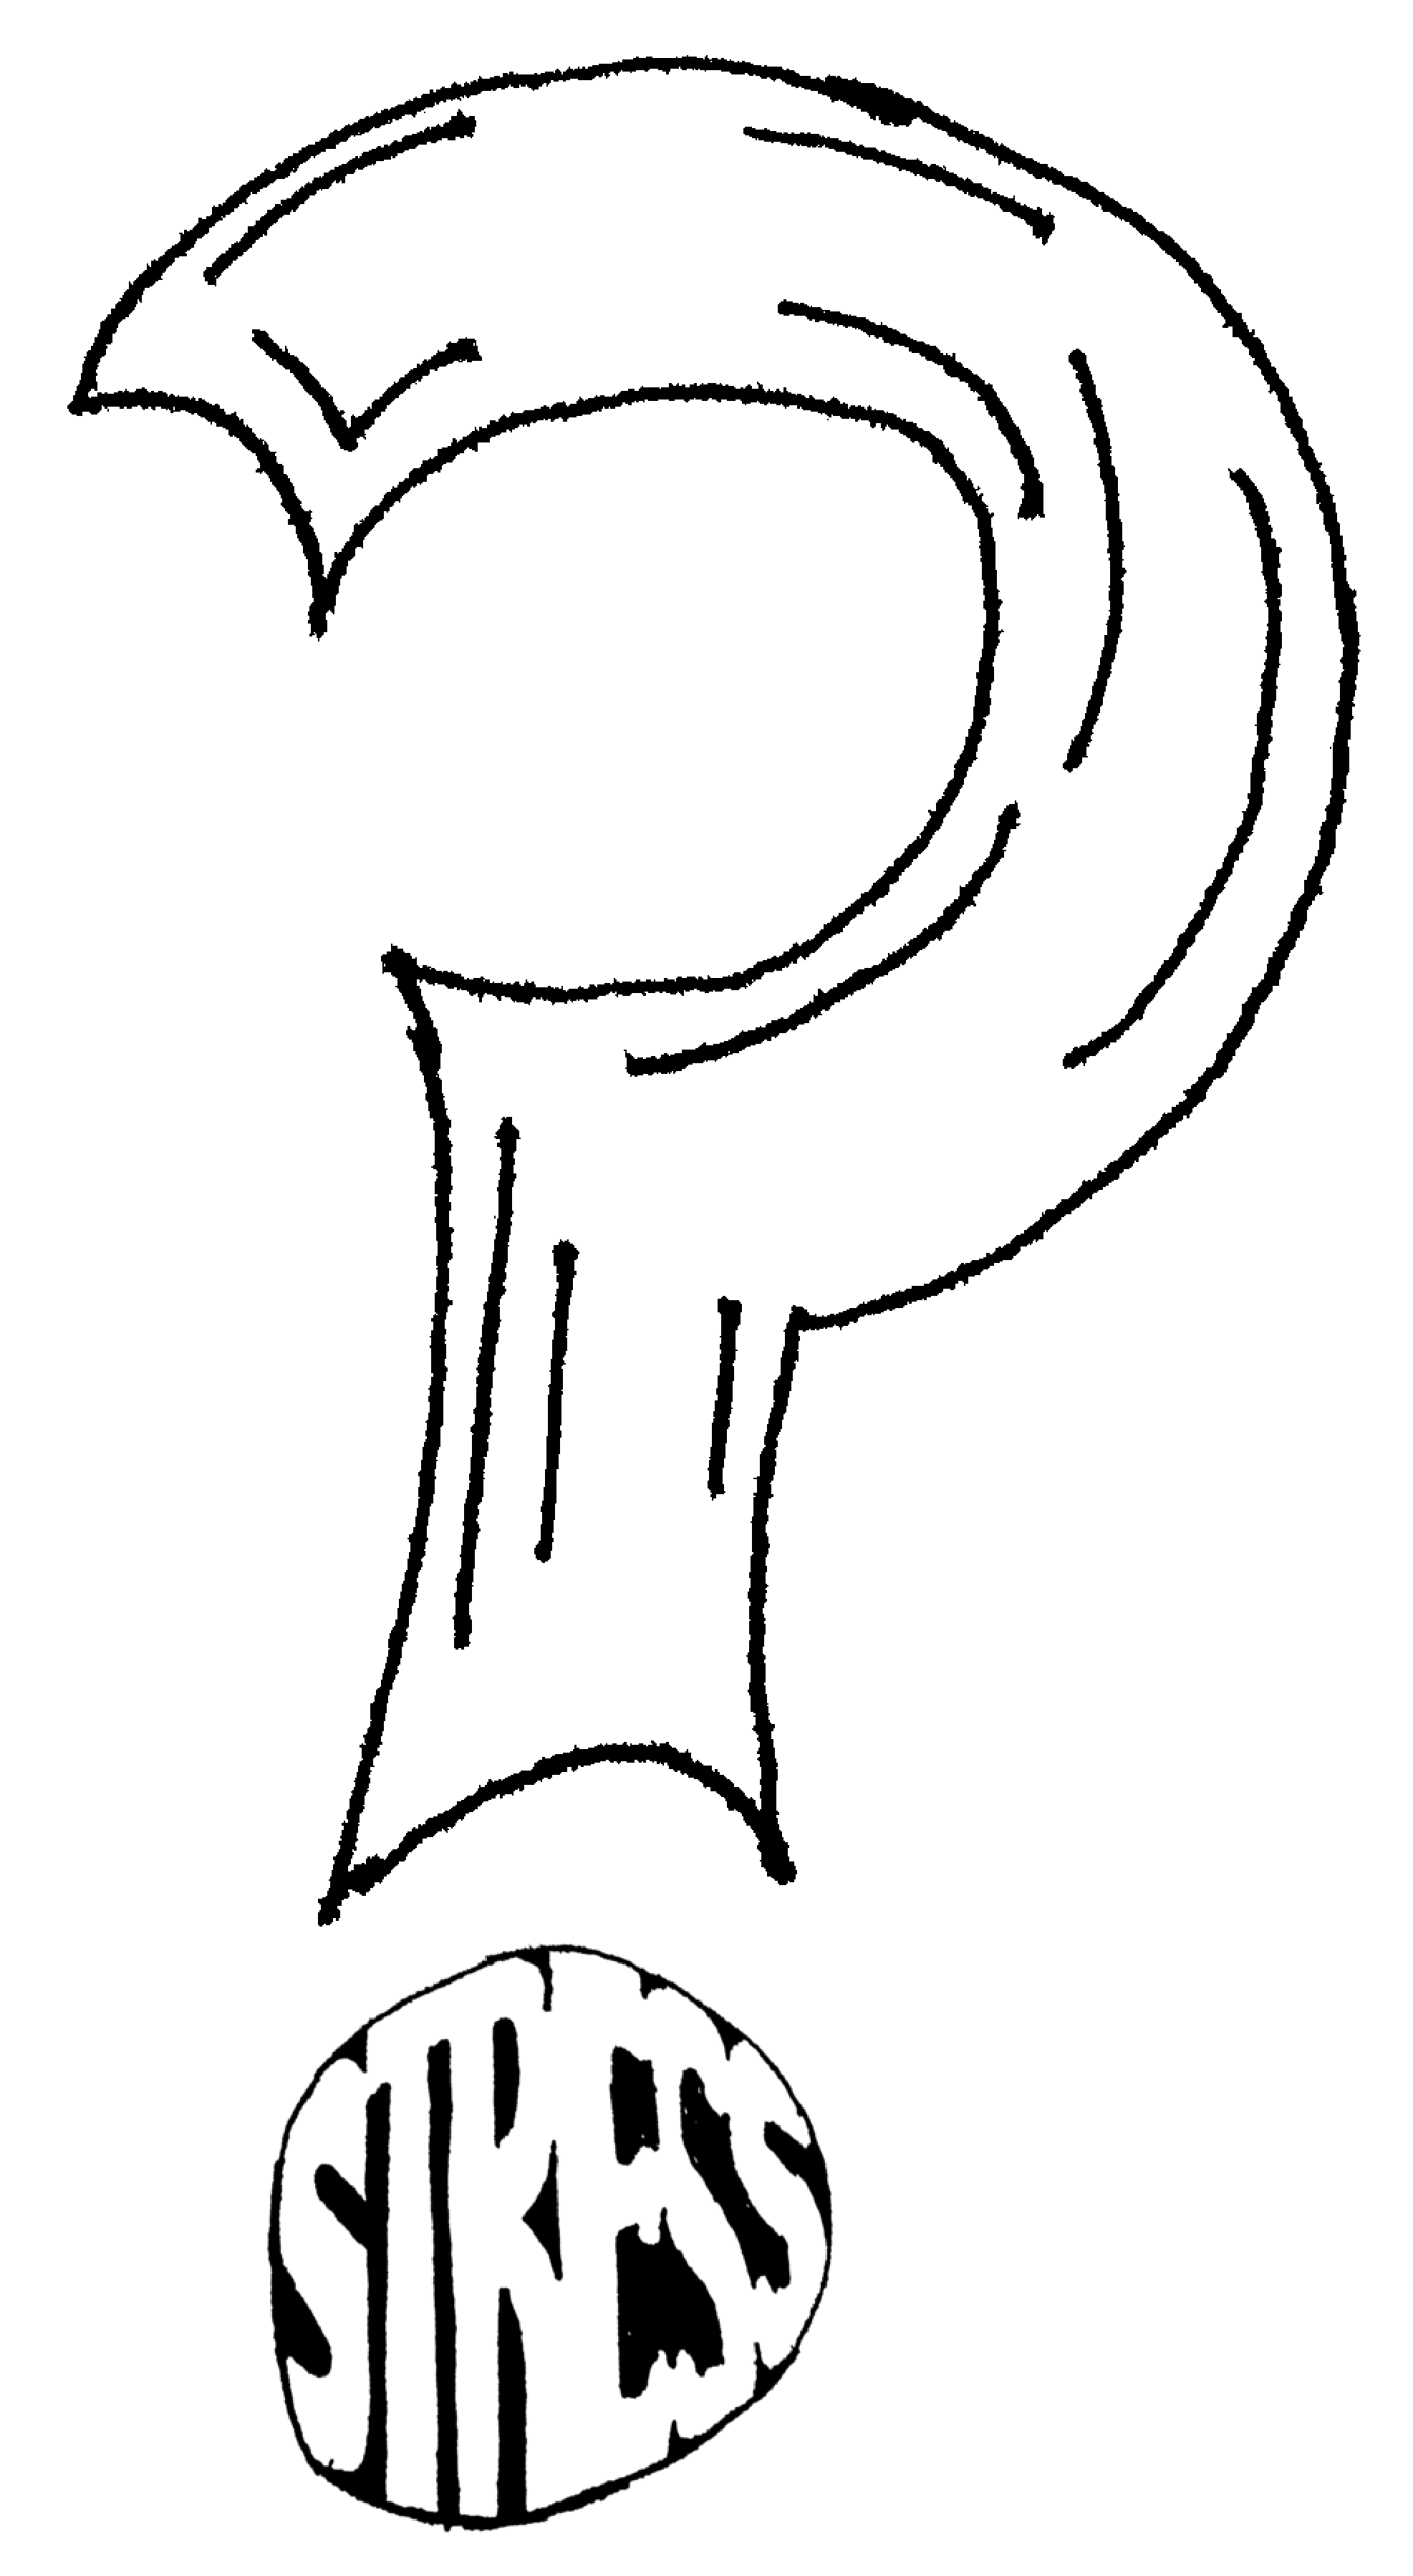
\includegraphics[width=\linewidth]{Question}
\column{0.7\textwidth} % Right column and width
\pause is stress in our: \ldots \pause
 \begin{itemize}
 \item<3, 6> \structure{Outside of us} (yelling person, time pressure, \ldots)?
 \item<4, 6>  \structure{Body} (muscles, nerves, nervous systems, heart, glands)?
 \item<5, 6>  \structure{Mind} (fight or flight, coping mechanism, adaptation)?
   \end{itemize}
\end{columns}
\end{frame}


\begin{frame}
\frametitle{Stress is unavoidable in life, \ldots}
\begin{columns}[c] % The "c" option specifies centered vertical alignment while the "t" option is used for top vertical alignment
\column{.3\textwidth} % Left column and width
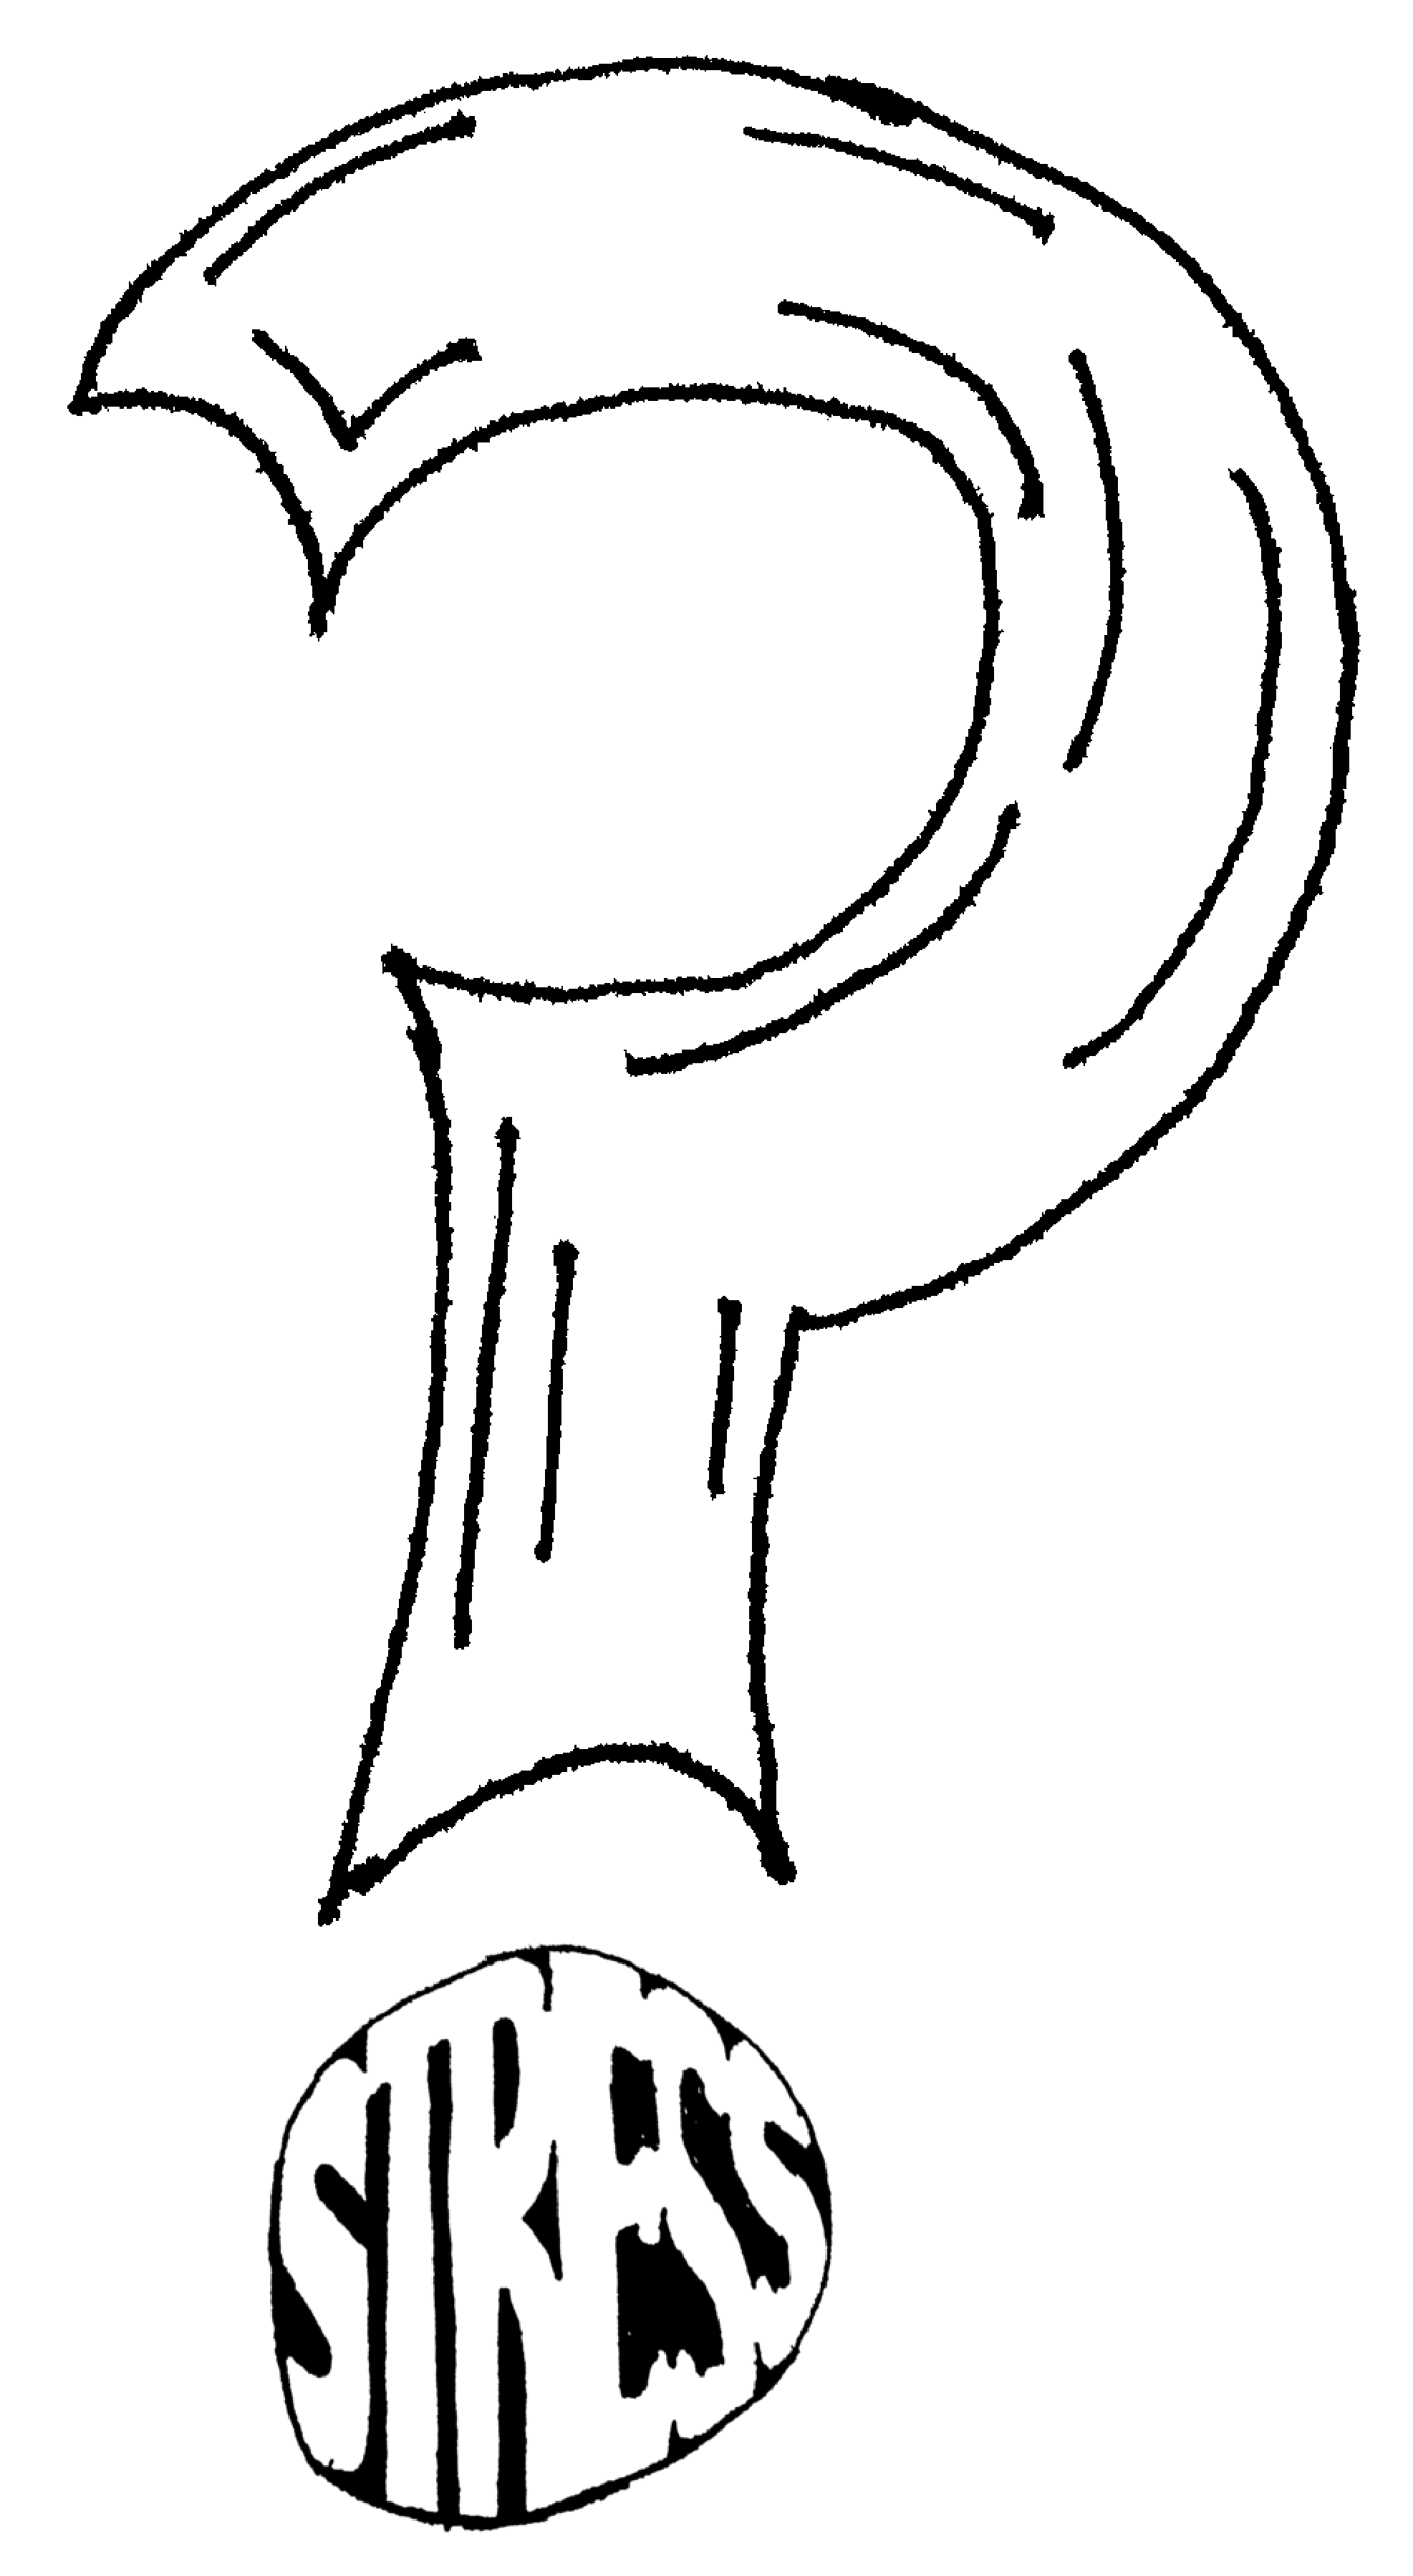
\includegraphics[width=\linewidth]{Question}
\column{0.7\textwidth} % Right column and width
\pause but can we do something? \ldots \pause
 \begin{itemize}
 \item<3, 9> \structure{Regulate}
 \item<4, 9> \structure{Negative stress} vs \structure{positive stress}
 \item<5, 9> \structure{Stress resistance} 
 \item<6, 9> \structure{Relaxation} and \structure{mindfulness} exercises
 \item<7, 9> \structure{Eat consciously}
 \item<8-9> A \structure{mindful life} 
 \end{itemize}
\end{columns}
\end{frame}



\end{document}